%!TEX TS-program = xelatex
%!TEX encoding = UTF-8 Unicode

\documentclass[12pt]{beamer}
\usepackage{amsmath, fancyvrb, textcomp}

%% Beamer 版面配置
\beamertemplatenavigationsymbolsempty % 去除 Beamer 導覽工具列
%\setbeamertemplate{footline}[frame number]{}
\mode<presentation>
\usetheme{Frankfurt}
%\usecolortheme{whale}
%\usetheme{Madrid}
\useinnertheme{circles}
%\usecolortheme{beaver}
%\usefonttheme{structurebold}

\DefineVerbatimEnvironment{MyVerbatim}{Verbatim}{fontsize=\tiny}

%% 西文字配置
\linespread{1.2}
\usepackage{arevmath}
\usepackage[no-math]{fontspec}
\setmainfont[Mapping=tex-text,LetterSpace=0]{Fira Sans Book}
\setsansfont[Mapping=tex-text,LetterSpace=0]{Fira Sans Book}
\setmonofont{Inconsolata}
\usefonttheme{professionalfonts}

%% 中文字配置
\usepackage[
  CJKmath=true, indentfirst=false, PunctStyle={quanjiao}, CheckSingle=false,
  CJKecglue = {\hskip 0.15em}
]{xeCJK}
\setCJKmainfont[Scale=1,BoldFeatures={FakeBold=2}]{Heiti TC Medium}
\setCJKmonofont[Scale=1,BoldFeatures={FakeBold=2}, FakeStretch=1]{Heiti TC Light}

\title[初學者學習R語言]{初學R語言的100分鐘}
\author[廖鎮磐]{廖鎮磐 \\ \texttt{<andrew.43@gmail.com>}\\ 東海大學生命科學系}
\institute{\normalsize 2015年3月15日於蓮華池}
\date{\scriptsize 
\includegraphics[width=1in]{cc.pdf}\\[5pt]
本文件採用姓名標示-相同方式分享 4.0 國際(CC BY-SA 4.0;詳細內容請見 \url{http://creativecommons.org/licenses/by-sa/4.0/deed.zh_TW})。\\ 本文件之PDF副本可於 \url{} 下載。}



\AtBeginSection[] {
  \begin{frame}
    \frametitle{大綱}
    \tableofcontents[currentsection]
  \end{frame}
  \addtocounter{framenumber}{-1}
} 

\begin{document}

\begin{frame}
\titlepage
\end{frame}

\begin{frame}
\frametitle{大綱}
\tableofcontents
\end{frame}

\section{事前準備}\subsection{}

\begin{frame}{初學R}
\begin{block}{特性}
\begin{itemize}
\item 自由、免費、跨平台。
\item 是一種「程式語言」,像Python、Perl、JAVA等。
\item 是一種「統計工具」,像SAS、SPSS等。
\item 強大的視覺化工具,畫專業的圖,但需要經驗。
\end{itemize}
\end{block}
\begin{block}{怎麼入門?}
\begin{itemize}
\item 買(可能不只一本)書。
\item 網路教學和論壇。
\end{itemize}
\end{block}
\end{frame}

\begin{frame}[fragile]{安裝R語言}
\begin{enumerate}
\item 到達\texttt{http://www.r-project.org/}
\item 點選Download, Packages (CRAN) \\
\item 選擇作業平台
	\begin{center}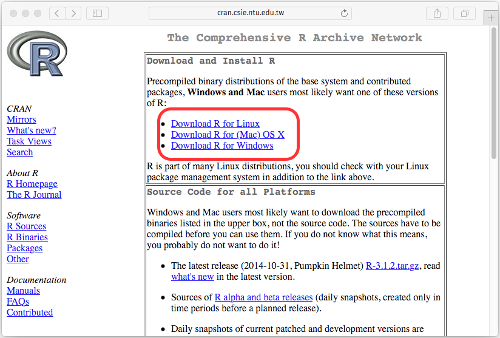
\includegraphics[width=0.7\textwidth]{downloadR.png}\end{center}
\end{enumerate}
\end{frame}


\begin{frame}[fragile]{安裝R的套件}
\begin{block}{什麼是套件(package)?}
\begin{itemize}
\item 安裝在R系統裡的外掛。
\item 不用「重新造輪子」。
\item 和R一樣,大多都可自由使用。
\end{itemize}
\end{block}

\begin{block}{如何安裝套件?}
\begin{enumerate}
\item 有網路。
\item \verb+install.packages("套件名稱") #安裝某套件+
\item \verb+update.packages() #更新所有已安裝套件+
\end{enumerate}
\end{block}
\end{frame}

\section{小試身手}\subsection{}

\begin{frame}[fragile]{計算機}
\begin{verbatim}
> 2.4 + 42
[1] 44.4
> sqrt(100)
[1] 10
\end{verbatim}
\end{frame}


\end{document}